\documentclass{beamer}
\usepackage{graphicx}
\usepackage{listings} % Syntax highlighing
\usepackage{fancyvrb} % Inline verbatim
\usepackage{hyperref} % Hyperlinks
\hypersetup{pdfpagemode=FullScreen}
\usepackage{tikz}

\usetheme{Boadilla}
\title{Yara Rules}
\author{UMBC Malware Data Science}
\date{Week 13: 28 April 2020}

\begin{document}

\begin{frame}{Recap}
    We've spent most of the course looking at malware samples, and creating models. There are other uses for $n$-grams.
\end{frame}

\begin{frame}{Yara Rules}
    \only<1>{
        \begin{itemize}
            \item YARA: Another Recursive Acronym
            \item Yet Another Ridiculous Acronym
            \item Created in 2013 by Victor Alvarez \href{https://twitter.com/plusvic}{@plusvic} at \href{https://www.virustotal.com/}{VirusTotal}.
            \item Yara is an advanced pattern matching language for finding malware, and it can do some parsing of executables files.
            \item It's open source, works with C/C++ \& Python. \url{https://github.com/VirusTotal/yara}.
        \end{itemize}
    }
    \only<2>{
        \begin{itemize}
            \item Match whole or parts of strings or byte sequences.
            \item Specify if strings or bytes should be at a specific location.
            \item Yara modules for math functions, ELF \& PE32 parsing, .NET-related items.
            \item Lots of examples at \url{https://github.com/Yara-Rules/rules}.
        \end{itemize}
    }
\end{frame}

\begin{frame}[fragile]{Yara Example}
    \begin{verbatim}
rule PoisonIvy_2 {
  meta:
    author = "Kevin Breen <kevin@techanarchy.net>"
    date = "2014/04"
    ref = "http://malwareconfig.com/stats/PoisonIvy"
    maltype = "Remote Access Trojan"
    filetype = "exe"
  strings:
    $stub = {04 08 00 53 74 75 62 50 61 74 68 18 04}
    $string1 = "CONNECT %s:%i HTTP/1.0"
    $string2 = "ws2_32"
    $string3 = "cks=u"
    $string4 = "thj@h"
    $string5 = "advpack"
  condition:
    $stub at 0x1620 and all of ($string*) or (all of them)
}
        \end{verbatim}
\end{frame}

\begin{frame}{Creating Rules}
    Creating these Yara rules might take an experienced analyst a few minutes, or perhaps several months, to craft a good, strong, robust yara rule for a malware sample, or malware family.
    \\ ~~ \\
    We've discussed how using hashing and integer arrays to keep track of $n$-grams speeds up the $n$-gram collecting processes, and enables collection of large $n$-grams ($n > 6$). We can create and store large $n$-grams for our malware \& goodware data, and use that to identify $n$-grams unique to a malware family.
    \\ ~~ \\
    So $n$-grams prevalent in the malware family which aren't in the common $n$-grams of the dataset as a whole might be candidate byte sequences for automatic Yara rule creation, and this can be done much faster than by hand.
    \\ But first...
\end{frame}

\begin{frame}{Bloom Filters}
    \only<1>{
        \begin{itemize}
            \item Bloom Filters are a probabilistic data structure first conceived by Burton Bloom in 1970.\footnote{\url{https://en.wikipedia.org/wiki/Bloom_filter}} They are used to determine if a given piece of data is in the set or not.
            \item Bloom Filters can have false positives, but \textit{not} false negatives. It can never say that data was previously inserted into the Bloom Filter when in fact it wasn't.
            \item When the Bloom Filter says data was provided, it's a probability, instead of an absolute.
            \item Bloom Filters don't store the data directly, but rather a compact representation of the data. As such, the original data cannot be retrieved from the Bloom Filter, you have to query the Bloom Filter with the data to see if it has been inserted.
            \item They are very useful when you're willing to sacrifice accuracy for speed or computability.
        \end{itemize}
    }
    \only<2>{
        We need a way to quickly, and using as little disk \& memory space as possible, to store all of these $n$-grams for various sizes of $n$.
        \\ ~~ \\
        Bloom Filters are just the data structure needed. Using hash functions, they can provide a probability of having the $n$-gram, but have zero chance of incorrectly indicating that an $n$-gram was inserted when it really wasn't (zero false positives).
        \\ ~~ \\
        \begin{columns}
            \column{0.5\textwidth} {
    $hash1(someInput) \mod{length} $\rightarrow$ 3$ \\
    ~$hash2(someInput) \mod{length} $\rightarrow$ 5$ \\
    ~$hash3(someInput) \mod{length} $\rightarrow$ 7$
            }
            \column{0.5\textwidth}{
                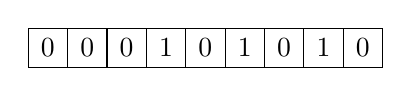
\begin{tikzpicture}[every node/.style = {shape          = rectangle,
                                             draw,                    %% here
                                             %double=red,              %% here
                                             %double distance =1pt,    %% here
                                             %fill           = black!30!white,
                                             minimum width  = 0.5cm,
                                             minimum height = 0.5cm,
                                             align          = center,                                         
                                             text           = black}]
                \node (0;0) at (0,0)   {0};
                \node (0;0) at (0.5,0) {0};
                \node (0;0) at (1,0)   {0};
                \node (0;0) at (1.5,0) {1};
                \node (0;0) at (2,0)   {0};
                \node (0;0) at (2.5,0) {1};
                \node (0;0) at (3,0)   {0};
                \node (0;0) at (3.5,0) {1};
                \node (0;0) at (4,0)   {0};
                \end{tikzpicture}
            }
        \end{columns}
        \\ ~~ \\
        Likelihood for a false positive is the likelihood of a collision on all hash functions used, and the likelihood of collisions can be reduced by increasing the array size.
    }
\end{frame}

\begin{frame}[fragile]{Bloom Filter in Python}
    \lstset{language=Python,
        basicstyle=\tiny,
        keywordstyle=\color{blue}\ttfamily,
        stringstyle=\color{red}\ttfamily,
        commentstyle=\color{green}\ttfamily,
        morecomment=[l][\color{magenta}]{\#}
}
\begin{lstlisting}
import os
import zlib
import pickle
import numpy as np

P_B = 227
P_M = 1000005

def rabin_hash(ngram):
    r = 0
    for ng in ngram:
        r = r * P_B + ord(ng)
        r %= P_M
    return abs(r)

def crc32_hash(ngram):
    if type(ngram) == str:
        ngram = ngram.encode()
    return abs(zlib.crc32(ngram))

def adler32_hash(ngram):
    if type(ngram) == str:
        ngram = ngram.encode()
    return abs(zlib.adler32(ngram))
\end{lstlisting}
\end{frame}

\begin{frame}[fragile]{Bloom Filter in Python}
    \lstset{language=Python,
        basicstyle=\tiny,
        keywordstyle=\color{blue}\ttfamily,
        stringstyle=\color{red}\ttfamily,
        commentstyle=\color{green}\ttfamily,
        morecomment=[l][\color{magenta}]{\#}
}
\begin{lstlisting}
import pickle
import numpy as np

class BloomFilter:
    def __init__(self, length=0, fname=None):
        if fname is not None:
            with open(fname, "rb") as f:
                tempDict = pickle.load(f)
            self.bits = tempDict["bits"]
            self.length = len(self.bits)
        else:
            self.length = length
            self.bits = np.zeros(length, dtype=np.bool)
        self.hash_functions = (rabin_hash, crc32_hash, adler32_hash)

    def insert(self, data):
        for func in self.hash_functions:
            index = func(data) % self.length
            self.bits[index] = True

    def contains(self, data):
        for func in self.hash_functions:
            index = func(data) % self.length
            if self.bits[index] == False:
                return False
        return True

    def isempty(self):
        return np.sum(self.bits) == 0

    def save(self, fname):
        tempDict = {"length": self.length, "bits": self.bits}
        with open(fname, "wb") as f:
            pickle.dump(tempDict, f)
\end{lstlisting}
\end{frame}

\begin{frame}{Bloom Filter Implementations}
    It's better to find an existing implementation, than trying to create your own. For Python, a good example is on PyPi: \url{https://pypi.org/project/bloom-filter/}.
    \\ ~~ \\
    One for Go: \url{https://github.com/willf/bloom}.
    \\ ~~ \\
    Go is mentioned because it will run much faster over larger sets of data. Go ahead, ask me how I know.
    \pause
    \\ ~~ \\
    My Go code finished creating Bloom Filters from over 2 million goodware/malware samples for $n$-grams for sizes of 8, 16, 32, 64, 128, 512 in the time that my Python code took to get partially through the 8-grams, and never finished. This is with the Python code using \texttt{multiprocessing} and Go implementation using multiple threads.
\end{frame}

\begin{frame}{Strategy}
    \begin{enumerate}
        \item Find $n$-grams of various sizes over the entire collection of goodware \& malware, save into a different Bloom Filter for each size, save to disk.
        \item Find large $n$-grams in the collection of files
        \item Keep track of $n$-grams in common to all files, or sets of $n$-grams which provide coverage over all files ($n$-gram $A$ might match files 1, 2, 3 and $n$-gram $B$ might match files 4, 5, 6.)
        \item Remove $n$-grams which have been found in the Bloom Filters.
        \item Save the remaining $n$-grams as a Yara rule, with a preference for larger $n$-grams, or for adjacent or overlapping $n$-grams.
        \item Test the resulting Yara rule on your data. If there are no remaining $n$-grams, your malware family may be too diverse for one Yara rule, or may not be \textit{one} family. Sometimes so-called malware families are actually common toolkits used by an adversary, but don't share common code.
    \end{enumerate}
\end{frame}

\begin{frame}{Algorithmically-Created Rules}
    A drawback of this method is that the $n$-grams might have come from non-executable portions of the file, and that the person looking at the Yara rule doesn't know why a particular byte sequence was chosen.
    \\ ~~ \\
    Most malware reverse engineers prefer rules which represent the functionality of the sample(s), due to two \textit{assumptions}: executable sections are unlikely to change too much for a given malware family, and this yields fewer false positives.
    \\ ~~ \\
    All are valid concerns, but producing Yara rules faster might be worth the trade-off.
\end{frame}

\begin{frame}{Lab 13}
    Using the provided Bloom Filter code and serialized Bloom Filters, find sequences of bytes which exist in a chosen the Ember 2018 malware family, but are not in the Bloom Filters representing the dataset overall.
\end{frame}

\end{document}